\documentclass[a4paper]{article}

\usepackage[utf8]{inputenc}


\title{\textbf{Práctica 4: Fundamentos de la ciencia de datos}}
\author{Luis Alejandro Cabanillas, Alvaro de las Heras, Mohssin Nagib Najim}

\usepackage{Sweave}
\begin{document}
\Sconcordance{concordance:Practica4.tex:Practica4.Rnw:%
1 8 1 1 0 9 1 1 2 1 0 1 1 14 0 1 2 2 1 1 2 1 0 1 1 8 0 1 2 14 1 1 2 9 0 %
1 2 4 1 1 2 24 0 1 2 6 1 1 2 15 0 1 2 2 1 1 2 10 0 1 1 10 0 1 2 2 1 1 2 %
10 0 1 1 10 0 1 2 6 1 1 2 1 0 3 1 3 0 1 2 3 1 1 4 3 0 1 2 1 0 1 1 3 0 1 %
2 1 1 1 2 1 0 3 1 1 2 1 0 2 1 3 0 1 2 3 1 1 3 2 0 1 1 1 2 1 0 3 1 1 3 1 %
0 1 1 3 0 1 2 1 3 6 0 1 2 1 3 6 0 1 2 2 1 1 2 4 0 1 2 1 3 6 0 1 2 3 1 1 %
4 3 0 1 2 1 0 1 2 1 0 1 1 3 0 1 2 2 1 1 2 1 0 4 1 4 0 1 2 3 1 1 2 1 0 2 %
1 1 2 1 0 1 2 1 0 1 2 4 0 2 2 5 0 1 2 3 1 1 2 1 0 1 2 1 0 2 1 1 3 6 0 1 %
1 5 0 1 4 4 0 1 5 7 0 1 2 3 1 1 2 1 0 1 1 3 0 1 3 5 0 1 2 3 1}



\maketitle

\section{Ejercicio 1}La primera parte de la práctica consistirá en la realización de un ejercicio en clase, en el que se llevará a cabo un análisis de clasificación no supervisada de datos con R aplicando todos los conceptos vistos en el tema. Este ejercicio se resolverá con algoritmo K-means y será el mismo problema que el visto en la descripción teórica del tema.

\subsection{Preparación de los datos y elección de los centroides}Lo primero que tendremos que hacer es introducir la matriz de muestra de los datos en R, para ello hacemos uso de la función \textbf{matrix}, utilizada ya en prácticas anteriores, y hacemos su traspuesta para tener los datos correctamente:

\begin{Schunk}
\begin{Sinput}
> m <- matrix(c(4,4,3,5,1,2,5,5,0,1,2,2,4,5,2,1),2,8)
> (m <- t(m))
\end{Sinput}
\begin{Soutput}
     [,1] [,2]
[1,]    4    4
[2,]    3    5
[3,]    1    2
[4,]    5    5
[5,]    0    1
[6,]    2    2
[7,]    4    5
[8,]    2    1
\end{Soutput}
\end{Schunk}

Una vez tenemos la muestra de datos en R, tenemos que elegir cuantos clusters habrá y los centroides de dichos clusters. Como tenemos una muestra con ocho pares de datos, lo más lógico es pensar que tendremos dos clusters. Los centroides se eligen arbitrariamente por el usuario, así que en este caso elegiremos de forma aleatoria c1(0,1), como centroide 1, y c2(2,2), como centroide 2. En R lo escribimos de forma similar al paso anterior: metemos los centroides en una matriz y hacemos la traspuesta de esta para tenerlos correctamente.

\begin{Schunk}
\begin{Sinput}
> centroides <- matrix(c(0,1,2,2),2,2)
> (centroides <- t(centroides))
\end{Sinput}
\begin{Soutput}
     [,1] [,2]
[1,]    0    1
[2,]    2    2
\end{Soutput}
\end{Schunk}

\subsection{Aplicación del algoritmo K-means}Ya tenemos todo lo que necesitamos para aplicar el algoritmo K-means en R. Este algoritmo tiene una función correspondiente en R (kmeans), que se estructura de la siguiente manera:
\begin{equation}
kmeans(m, centers, iter.max)
\end{equation}

Donde:
\begin{itemize}
	\item \textbf{{M:}} Es la matriz donde se encuentra la muestra de datos.
	\item \textbf{{Centers:}} Representa la matriz con los centroides elegidos.
	\item \textbf{{Iter.max:}} Número máximo de iteraciones permitidas.
\end{itemize}

Para usar la función tenemos que asegurarnos de tenerla cargada en el entorno de R. La función kmeans se encuentra en el paquete \textbf{stats}, que se carga por defecto cada vez que abrimos R. Para comprobarlo hacemos search():

\begin{Schunk}
\begin{Sinput}
> search()
\end{Sinput}
\begin{Soutput}
[1] ".GlobalEnv"        "package:stats"     "package:graphics" 
[4] "package:grDevices" "package:utils"     "package:datasets" 
[7] "package:methods"   "Autoloads"         "package:base"     
\end{Soutput}
\end{Schunk}

Como podemos ver, el paquete stats está cargado en nuestro entorno de R.

Ahora podemos aplicar kmeans. M será nuestra matriz m, donde tenemos cargada la matriz de muestra; centers será centroides, la matriz que almacena los centroides arbitrarios elegidos y en iter.max pondremos 4, ya que hemos realizado este ejercicio en la clase de teoría y sabemos que se va allevar a cabo en menos de 4 iteraciones. Así:

\begin{Schunk}
\begin{Sinput}
> (clasificacionns = kmeans(m, centroides, 4))
\end{Sinput}
\begin{Soutput}
K-means clustering with 2 clusters of sizes 4, 4

Cluster means:
  [,1] [,2]
1 1.25 1.50
2 4.00 4.75

Clustering vector:
[1] 2 2 1 2 1 1 2 1

Within cluster sum of squares by cluster:
[1] 3.75 2.75
 (between_SS / total_SS =  84.8 %)

Available components:

[1] "cluster"      "centers"      "totss"        "withinss"     "tot.withinss"
[6] "betweenss"    "size"         "iter"         "ifault"      
\end{Soutput}
\end{Schunk}

Como podemos ver, hemos obtenido dos centroides, uno por cada cluster. El primer centroide será (1.25, 1.5) y el segundo (4.00, 4.75), los mismos que hemos obtenido en la clase de teoría realizando el ejercicio a mano. También hemos obtenido un "Clustering vector", que nos dice en qué cluster está cada uno de los puntos de la muestra.

Una vez tenemos los centroides y el clustering vector, dividimos los datos en los dos clusters que hemos obtenido en el siguiente paso.

\subsection{División de los datos en clusters}Hemos obtenido dos clusters, ya que vemos que en el clusterin vector solo tenemos dos valores (1 y 2), que corresponden con la posición de los puntos de la muestra. Así, para saber a qué cluster pertenece cada punto, concatenaremos el clustering vector y m con \textbf{cbind}:

\begin{Schunk}
\begin{Sinput}
> (m = cbind(clasificacionns$cluster,m))
\end{Sinput}
\begin{Soutput}
     [,1] [,2] [,3]
[1,]    2    4    4
[2,]    2    3    5
[3,]    1    1    2
[4,]    2    5    5
[5,]    1    0    1
[6,]    1    2    2
[7,]    2    4    5
[8,]    1    2    1
\end{Soutput}
\end{Schunk}

Ahora tenemos una matriz m en la que aparece en la primera columna a qué cluster pertenece cada punto y en las otras dos columnas la posición x e y de cada suceso. Para obtener los dos clusters separados tendremos que obtener por un lado las filas de la matriz que tienen un 1 en la primera columna y, por otro, las que tienen un 2:

\begin{Schunk}
\begin{Sinput}
> (mc1 = subset(m,m[,1]==1))
\end{Sinput}
\begin{Soutput}
     [,1] [,2] [,3]
[1,]    1    1    2
[2,]    1    0    1
[3,]    1    2    2
[4,]    1    2    1
\end{Soutput}
\begin{Sinput}
> (mc2 = subset(m,m[,1]==2))
\end{Sinput}
\begin{Soutput}
     [,1] [,2] [,3]
[1,]    2    4    4
[2,]    2    3    5
[3,]    2    5    5
[4,]    2    4    5
\end{Soutput}
\end{Schunk}

Una vez tenemos los datos divididos, limpiamos cada matriz quitando la primera columna para tener solamente los puntos en cada cluster:

\begin{Schunk}
\begin{Sinput}
> (mc1 = mc1[,-1])
\end{Sinput}
\begin{Soutput}
     [,1] [,2]
[1,]    1    2
[2,]    0    1
[3,]    2    2
[4,]    2    1
\end{Soutput}
\begin{Sinput}
> (mc2 = mc2[,-1])
\end{Sinput}
\begin{Soutput}
     [,1] [,2]
[1,]    4    4
[2,]    3    5
[3,]    5    5
[4,]    4    5
\end{Soutput}
\end{Schunk}

Ya tenemos los dos clusters con los puntos que pertenecen a cada uno, por lo que hemos finalizado el ejercicio.

\section{Ejercicio 2}
En este ejercicio vamos a aplicar técnicas de clustering a un dataset de coches usados. Este dataset se ha obtenido en Kaggle, y recopila 1,5 GB de datos de coches en venta en la página de Craiglist. Las técnicas que se han aplicado son K-means, K-medoids, K-medians, DBSCAN, Clasificación Jerárquica Aglomerativa y K-means jerarquico. Con cada análisis además se visualizarán los datos.
\subsection{Preparación y carga de datos} El primer paso a realizar es la carga de las bibliotecas que nos permiten ejecutar los algoritmos y visualizar los datos. Para visualizar los datos se usará \textbf{factoextra} y el propio \textbf{plot}, y para los algoritmos \textbf{cluster} (K-means y K-medoids), \textbf{Gmedian} (K-median) y \textbf{dbscan} (DBSCAN).

\begin{Schunk}
\begin{Sinput}
> library("factoextra")
> library("cluster")
> library("Gmedian")
> library("dbscan")
\end{Sinput}
\end{Schunk}

Los datos que teníamos eran demasiado grandes(1,5GB), por lo que hemos troceado el CSV en otros de menor tamaño. Para agilizar la carga de datos, solo hemos elegido los que nos interesaban relativos a los coches, quitando algunos redundantes como descripciones o URLs, esto se ha hecho con el parámetro \textbf{colClasses} que recibe un vector con el tipo de cada columna, siendo NULL el valor que descarta la columna.    

Como los datos se han recogido con scraping hay muchos campos nulos o con cadenas vacías, como solución a este problema hemos puesto el parámetro \textbf{na.strings}, en el indicamos que remplace las cadenas con NA. Luego para asegurar que estuvieran todos los datos rellenos hemos usado \textbf{complete.cases}, que selecciona aquellos con todas las columnas sin NA. Esto también se puede hacer con na.omit. 
\begin{Schunk}
\begin{Sinput}
> columnas<-c("NULL","character","NULL","numeric","numeric","character",
+ "character","character","character","character","numeric","character",
+ "character","NULL","character","character","character","character",rep("NULL",4))
> coches <- read.csv("cochesReducidoMediano.csv",head=T,sep=",",encoding = "UTF-8",
+           colClasses=columnas,na.strings=c("","NA"))
> cochesCompletos <-coches[complete.cases(coches), ]
\end{Sinput}
\end{Schunk}

También pondremos unos valores límites para evitar valores anómalos y elegir centroides comprendidos entre ellos. Los valores anómalos se eliminan con la función \textbf{subset} y las condiciones que han de tener unidas por and. Otros cambios que se hacen son indicar el número de clusters y seleccionar las columnas númericas para clusterizar de nuestro interés (precio y kilometraje).
\begin{Schunk}
\begin{Sinput}
> precioMinimo <- 299
> precioMaximo <- 200000
> kilometrajeMinimo <- 10
> kilometrajeMaximo <- 100000
> cochesAjustados <- subset(cochesCompletos, cochesCompletos[ , 2] > precioMinimo & 
+     cochesCompletos[ , 2] < precioMaximo & cochesCompletos[ , 9] > kilometrajeMinimo)
> nClusters <- 5
> cochesAjustados <- cochesAjustados[,c(2,9)]
\end{Sinput}
\end{Schunk}
\subsection{K-means}
En este punto se va a aplicar K-means, de una forma similar a la del ejercicio anterior, elegiendo unos centroides aleatorios al principio de los que se obtendrán los clusters. Un cambio que hemos hecho ha sido el algoritmo que utiliza K-means, cambiando al de Lloyd, puesto que este si que garantiza que se devuelven los clusters, aunque pueden hacer que no esten centrados correctamente. La última modificación que se ha hecho ha sido la normalización de los datos, mediante \textbf{scale} para los datos y \textbf{rnorm} para los centroides. La normalización de los datos suele mejorar el rendimiento, porque otorga la misma importancia a todas las variables evitando que haya datos que tengan un importancia desproporcionada, a partir de ahora trabajaremos con los datos normalizados.   

Por esto lo hemos aplicado, y como los resultados muestran el rendimiento ha mejorado, formando unos cluster más definidos y agrupados, de los que solo 2 se ven afectados por los valores más altos. Mientras que el clustering normal muestra unos clusters menos uniformes y definidos, en parte debido a que los datos no están correctamente proporcionados.
\begin{Schunk}
\begin{Sinput}
> # Calculo de centroides (Con y sin normalizar)
> set.seed(0)
> centroidesPrecios <- sample(precioMinimo:precioMaximo, nClusters, replace=FALSE)
> centroidesKilometrajes <- sample(kilometrajeMinimo:kilometrajeMaximo, 
+                        nClusters, replace=FALSE)
> centroides <- matrix(c(centroidesPrecios,centroidesKilometrajes),nClusters,2)
> centroides.normalizados <-matrix(c( rnorm(nClusters), rnorm(nClusters)),nClusters,2)
> coches.normalizados <- scale(cochesAjustados)
> # Calculo de K-means
> clusters <- kmeans(cochesAjustados, centroides, algorithm = "Lloyd", 9)
> clusters.normalizados <- kmeans(coches.normalizados, centroides.normalizados, 9)
\end{Sinput}
\end{Schunk}

\begin{Schunk}
\begin{Sinput}
> fviz_cluster(clusters, cochesAjustados ,repel = TRUE, ellipse.type = "convex",
+              geom = "point", main="K-means sobre precio y kilometraje")
\end{Sinput}
\end{Schunk}
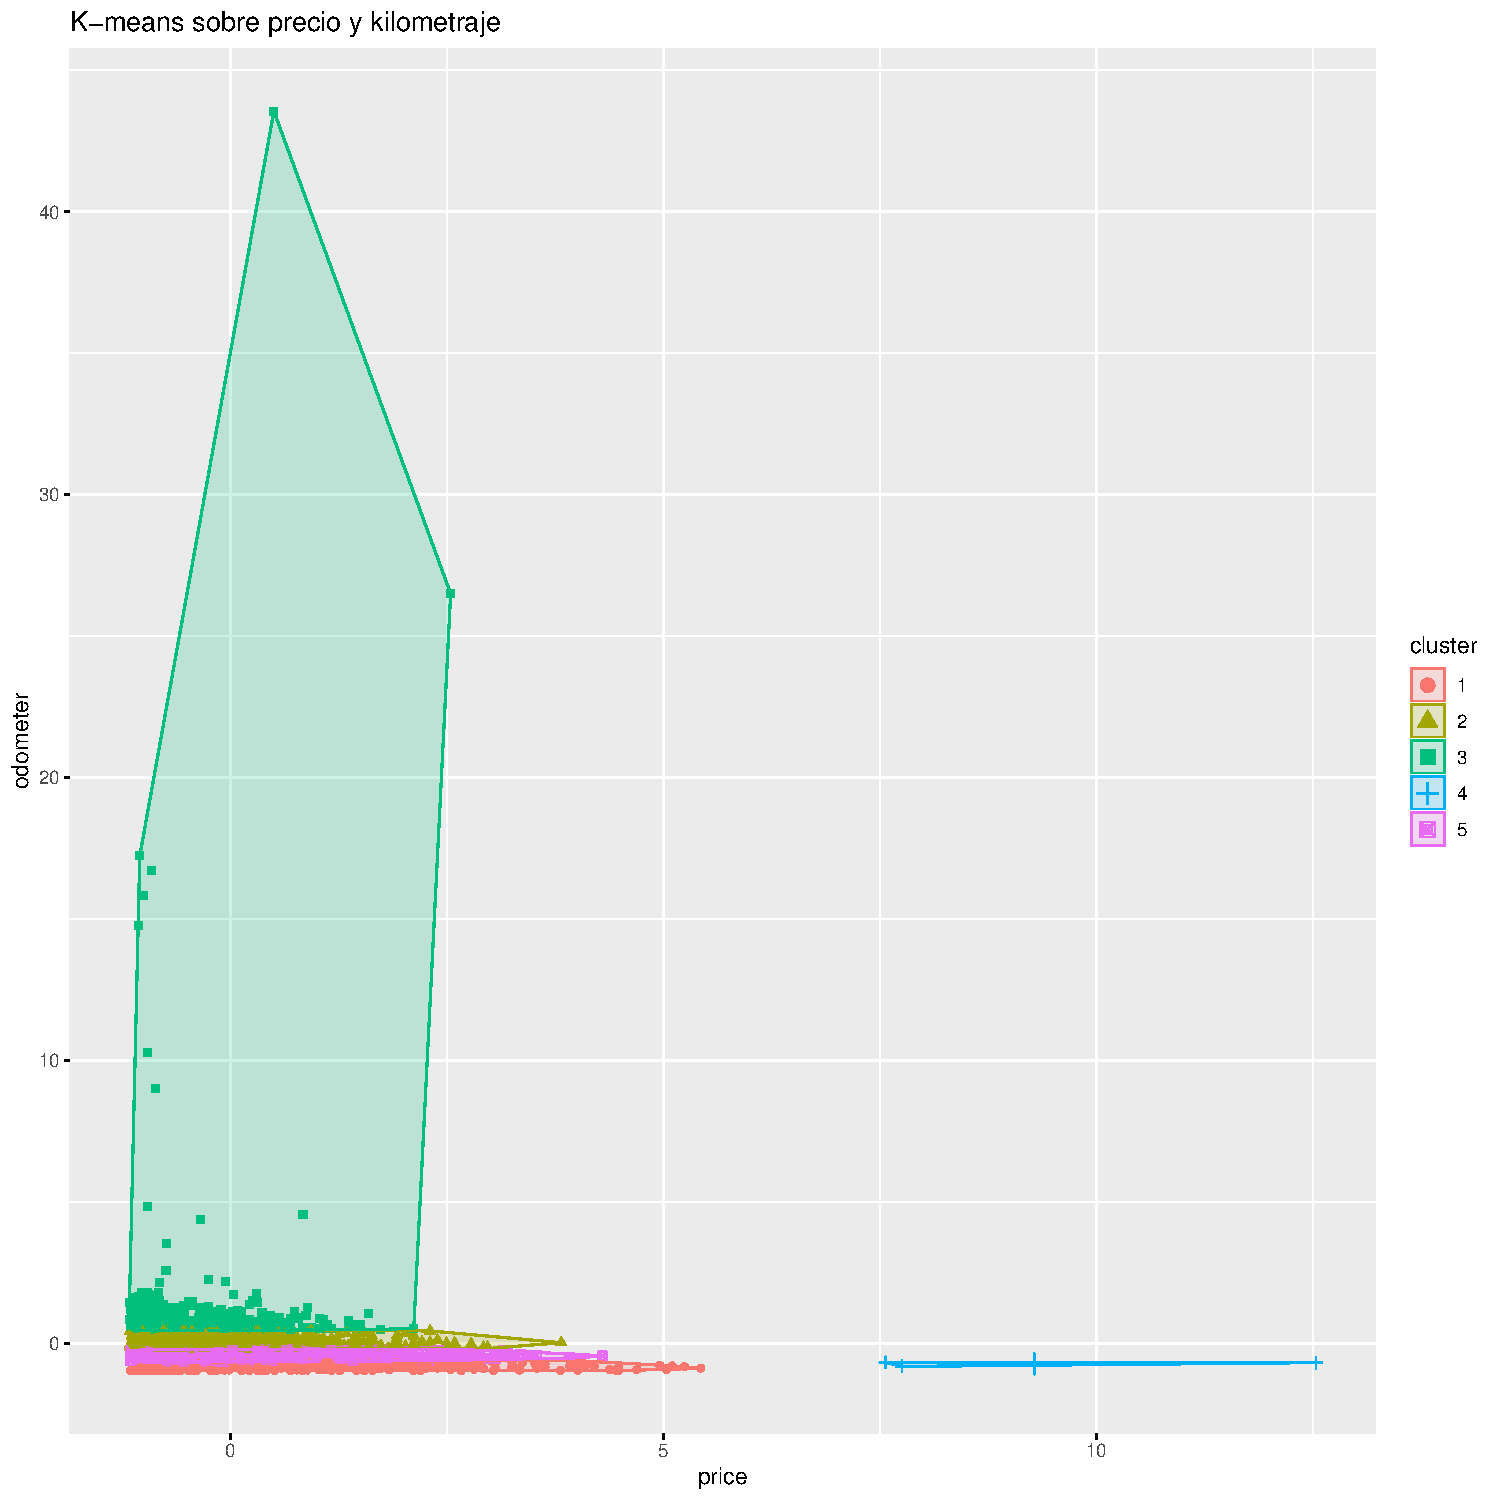
\includegraphics{Practica4-kmean}

\begin{Schunk}
\begin{Sinput}
> fviz_cluster(clusters.normalizados, coches.normalizados ,repel = TRUE, 
+              ellipse.type = "convex",geom = "point",main="K-means normalizado")
\end{Sinput}
\end{Schunk}
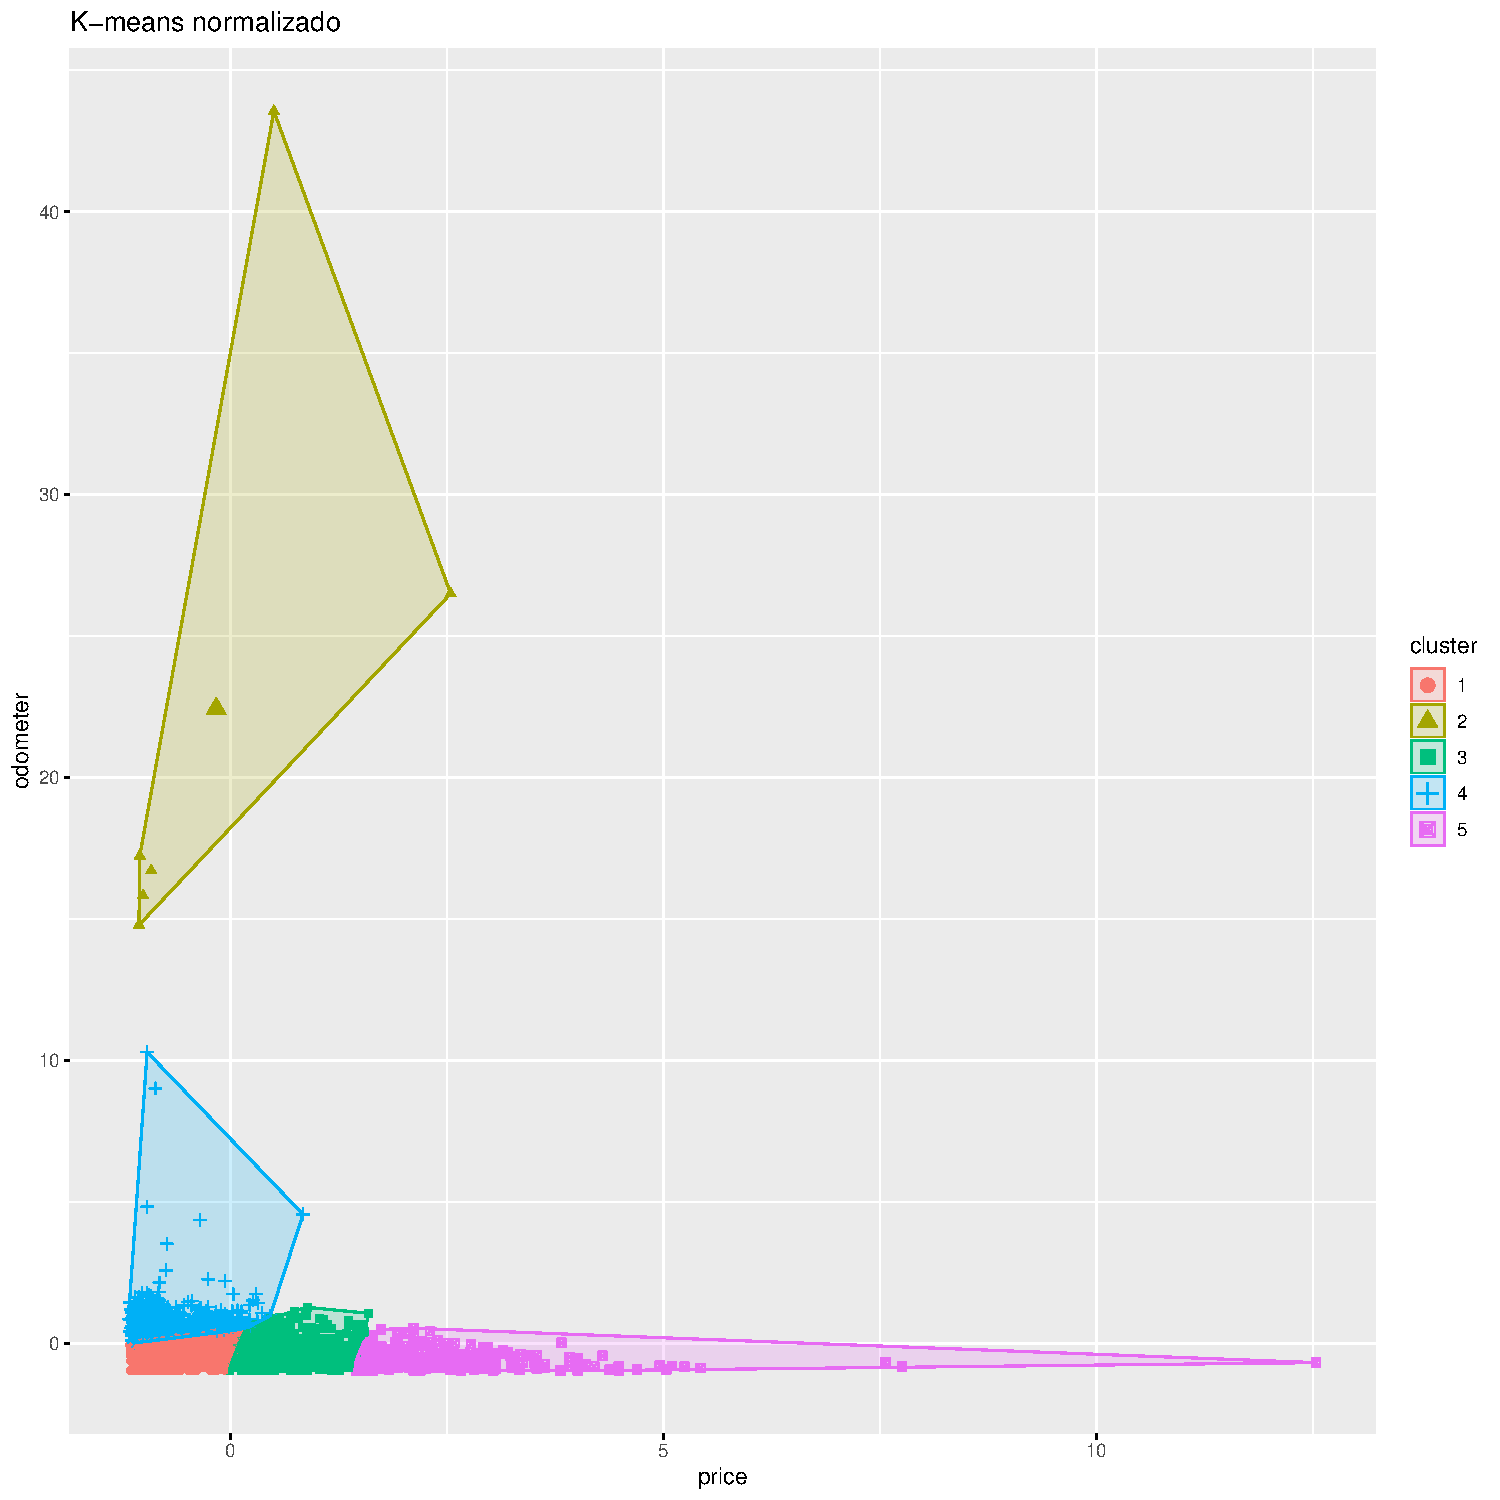
\includegraphics{Practica4-kmeannorm}

\subsection{K-medoids o PAM}
Se trata de un método de clustering similar al K-means, que también particiona pero difiere a la hora de escoger centros, porque los escoge de entre los puntos disponibles. Además, ofrece una mayor robustez al ruido y zonas aisladas y es más flexible aunque su coste computacional es bastante alto. El cálculo se realiza con el método \textbf{pam} de la biblioteca cluster.
\begin{Schunk}
\begin{Sinput}
> pam.res <- pam(coches.normalizados, nClusters)
\end{Sinput}
\end{Schunk}
El resultado es una clasificación buena al tener bien definidos y agrupados los clusters, a pesar de las partes aisladas, mejorando al K-means sin normalizar e igualando al normalizado.
\begin{Schunk}
\begin{Sinput}
> fviz_cluster(pam.res, geom = "point", ellipse.type = "convex",
+              main="K-medoids (PAM)")
\end{Sinput}
\end{Schunk}
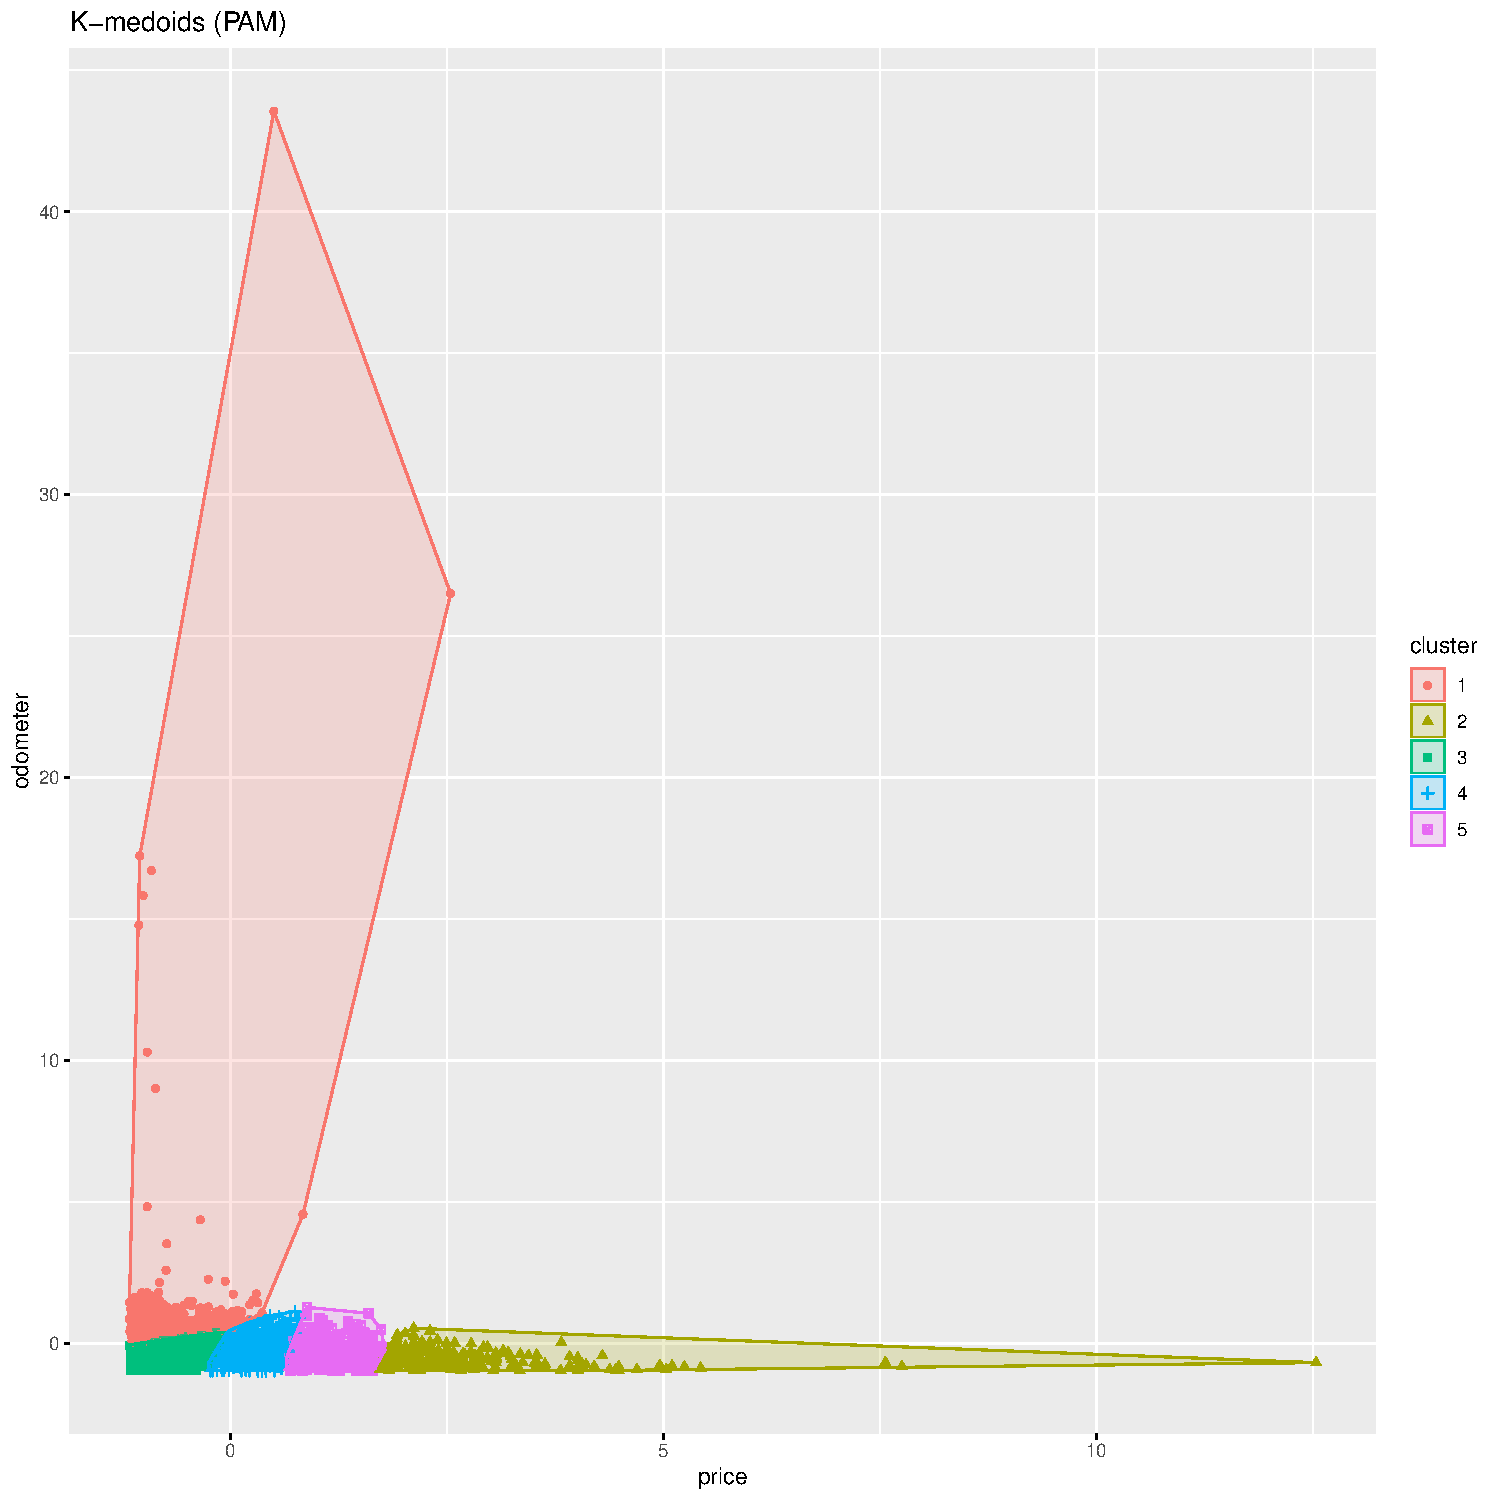
\includegraphics{Practica4-Kmedoids}
\subsection{K-median}
Otro método similar es el de K-median, este se caracteriza por el cálculo de la mediana, que equivale al cálculo de la distancia Manhattan frente a la euclídea del K-means. La ventaja que aporta es que tiende a agrupar mejor los datos especialmente si son valores enteros o binarios, al minimizar el error si lo comparamos con K-means, pero menos eficiente.

Para la realización de éste hemos utilizado la función \textbf{kGmedian} de la biblioteca Gmedian, a esta le hemos indicado el número de centros y le hemos pasado los datos normalizados, pero por problemas de eficiencia al tener tantos datos hemos tenido que reducirlo a 100 coches. 
\begin{Schunk}
\begin{Sinput}
> # Calculo de K-Median
> 
> cl.kmedian <- kGmedian(head(coches.normalizados,100), ncenters=nClusters)
> # Calculo de K-Mean para comparar resultados
> set.seed(1)
> centroides.normalizados <-matrix(c( rnorm(nClusters), 
+                                     rnorm(nClusters)),nClusters,2)
> cl.kmean <- kmeans(head(coches.normalizados,100), centroides.normalizados, 20)
\end{Sinput}
\end{Schunk}

Para facilitar su comparativa hemos simulado el problema igual pero con K-means,en las gráficas se puede ver como K-median agrupa en clusters más compactos y separados que K-means, mostrando así su eficacia.

\begin{Schunk}
\begin{Sinput}
> par(mfrow=c(2,1))
> plot(head(coches.normalizados,100), col = cl.kmedian$cluster, main="K-median")
> points(cl.kmedian$centers, col = 1:2, pch = 8, cex = 2)
> plot(head(coches.normalizados,100), col = cl.kmean$cluster, main="K-means")
> points(cl.kmean$centers, col = 1:2, pch = 8, cex = 2)
\end{Sinput}
\end{Schunk}
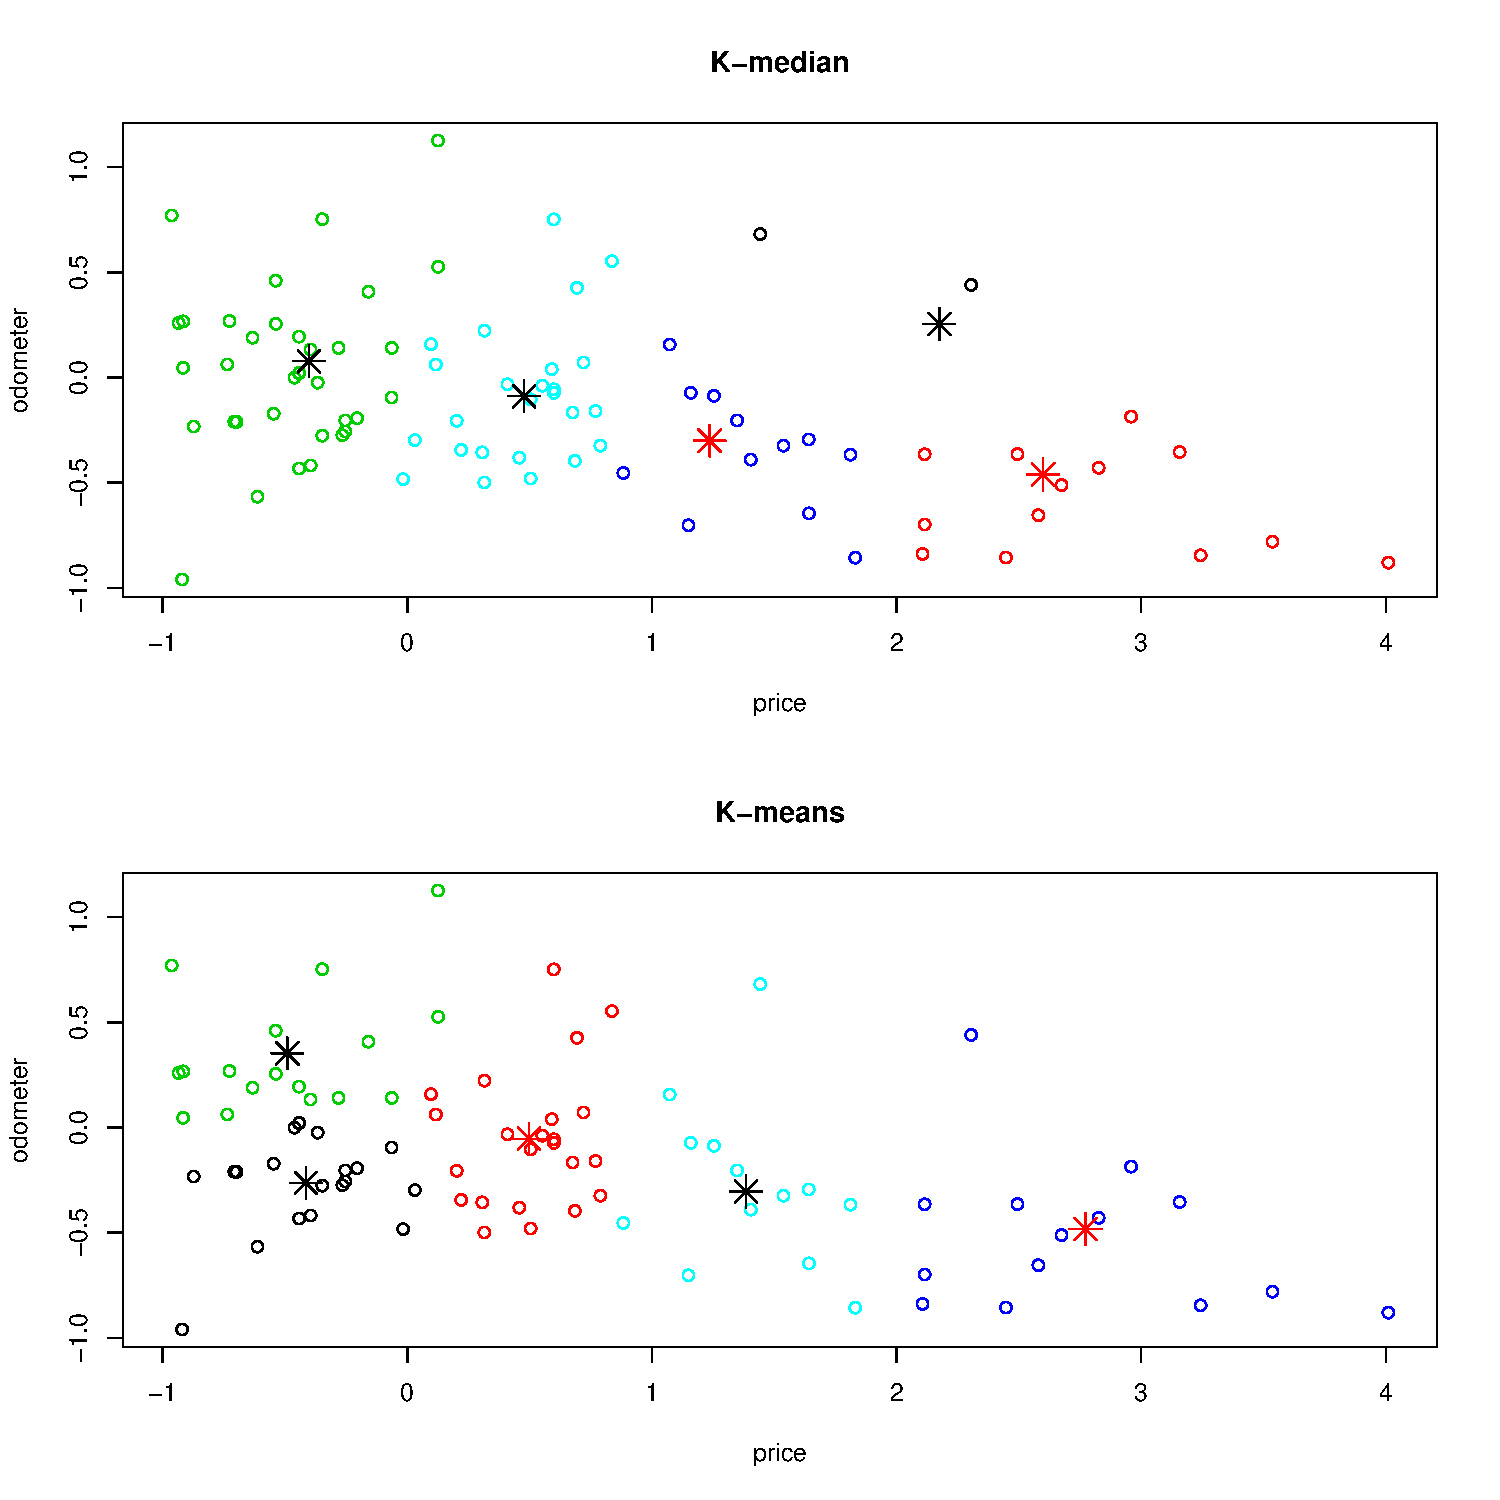
\includegraphics{Practica4-kmedian}
\subsection{DBSCAN}
El agrupamiento espacial basado en densidad de aplicaciones con ruido denominado DBSCAN, es muy distinto a los anteriores, de primeras no es necesario definir el número de clusters del problema lo cual supone una ventaja. Su funcionamiento consiste en ir visitando todos los puntos, para determinar si son posibles clusters. Un punto podrá ser un cluster si tiene suficientes vecinos (puntos.minimos) a una distancia Epsilon, de aquí viene el concepto de densidad. Si se trata de un cluster el proceso se repite con los nuevos puntos añadidos al inicial, cuando no haya más se comienza con otro punto nuevo. Se puede dar el caso de que haya puntos que no se encuentren en ningún cluster, estos son considerados ruido. La principal desventaja es que no siempre se puede aplicar porque hay problemas con densidad variable haciendo que no funcione correctamente.

La implementación se ha hecho con la biblioteca dbscan, y los métodos \textbf{KNNdistplot} y \textbf{dbscan.} kNNdistplot se usa para el cálculo de la epsilon, es un método de K-vecinos con el que calculamos la distancia media entre los puntos que se le indiquen. Una vez hemos calculado las distancias elegimos un epsilon que corte la gráfica justo en el punto en el que flexiona la gráfica, en este caso 0.2. Ya con los datos necesarios realizamos el dbscan, que nos arroja una gráfica en la que se deshace de todo el ruido, agrupando los puntos muy próximos en el cluster, siendo una clasificación muy buena mejorando considerablemente al resto, aunque se han formado algunos clusters de tamaño muy reducido.
\begin{Schunk}
\begin{Sinput}
> par(mfrow=c(1,1))
> puntos.minimos <- 3
> epsilon <- 0.2
> # Se obtiene epsilon para el DBSCAN y k = dim + 1
> dbscan::kNNdistplot(coches.normalizados, k =  puntos.minimos)
> # Epsilon coincide con la altura de la flexion de la linea
> abline(h = epsilon, lty = 2)
> # Se realiza el clustering con DBSCAN
> res.db <- dbscan::dbscan(coches.normalizados, epsilon, puntos.minimos)
\end{Sinput}
\end{Schunk}

\begin{Schunk}
\begin{Sinput}
> fviz_cluster(res.db, coches.normalizados, geom = "point")
\end{Sinput}
\end{Schunk}
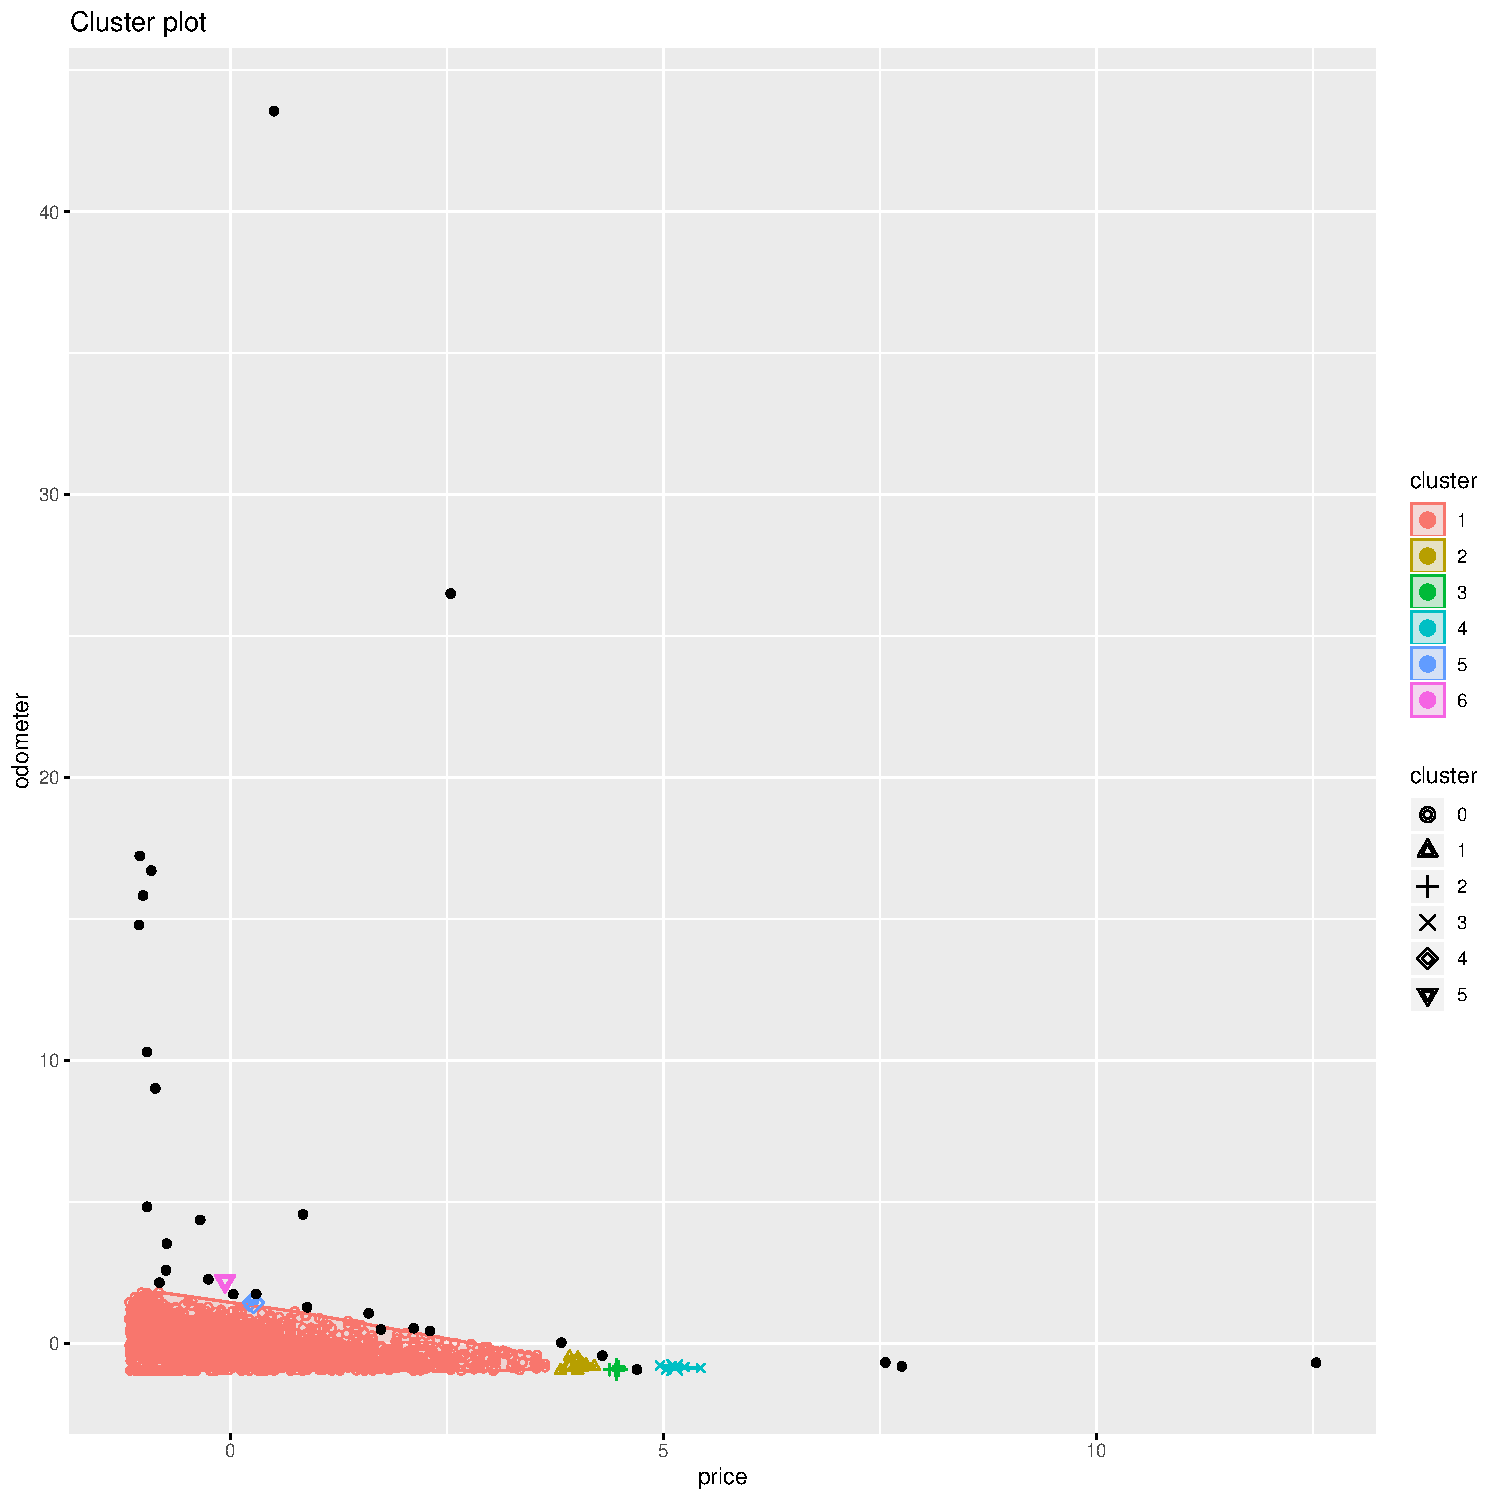
\includegraphics{Practica4-dbscan}

\subsection{Agrupación Jerárquica Aglomerativa}
La agrupación es una técnica para agrupar puntos de datos similares en un grupo y separar las diferentes observaciones en diferentes grupos, en este ejercicio como se ha explicado previamente se clasificará en función de el kilometraje y el precio. En el clustering jerárquico, los clusters se crean se manera que tengan un orden predeterminado, lo veremos en las gráficas numerado. Hay dos tipos, divisivo y aglomerativo, en este caso probaremos el aglomerativo, en el cual cada observación se asigna a su propio cluster, luego se calcula la distancia euclidiana entre cada uno de los clusters con la funcion \textbf{dist} y el método \textbf{"euclidean"}, y los dos clusters más similares se fusionan en uno, esta operación se irá iterando hasta que solo quede un grupo. Utilizando los datos que se han preparado previamente, representaremos gráficamente los clusters normalizados con los datos del dendograma que mejor correlación tengan, calcularemos con el método \textbf{"complete"} que corresponde al algoritmo MAX que define la proximidad entre los puntos más lejanos, y con el metodo \textbf{"average"} que corresponde con el algoritmo Group Average que define proximidad como la media de distancias entre todas las parejas que se puedan formar con puntos de los dos clusters. Para el cálculo de estos dendogramas haremos uso de la función \textbf{hclust}. Para el calculo de la correlación de cada uno haremos uso de la función \textbf{cor} para el calculo de la correlación y \textbf{cophenetic} para el cálculo de las distancias entre observaciones. Cuanto más cercano es el valor a 1, mejor refleja el dendrograma la verdadera similitud entre las observaciones. Valores superiores a 0.75 suelen considerarse como buenos, los dos métodos aplicados son buenos, pero utilizamos el de la media porque es el mejor. Esta medida puede emplearse como criterio de ayuda para escoger entre los distintos métodos:

\begin{Schunk}
\begin{Sinput}
> set.seed(102)
> #NORMALIZADO
> c <- dist(coches.normalizados, method = "euclidean")
> hc1 <- hclust(c, method = "complete")
> hc2 <- hclust(c, method = "average")
> #CORRELACION CON LOS METODOS COMPLETO Y CON LA MEDIA
> (cor(x = c, cophenetic(hc1)))
\end{Sinput}
\begin{Soutput}
[1] 0.806087
\end{Soutput}
\begin{Sinput}
> (cor(x = c, cophenetic(hc2)))
\end{Sinput}
\begin{Soutput}
[1] 0.915147
\end{Soutput}
\begin{Sinput}
> ##ASIGNAMOS CLUSTERS NORMALIZADOS
> clust <- cutree(hc2, k = 5)
\end{Sinput}
\end{Schunk}
\begin{Schunk}
\begin{Sinput}
> fviz_cluster(list(data = coches.normalizados, cluster = clust), 
+              geom = "point",
+              main="Agrupación Jerárquica Aglomerativa Clusters")
\end{Sinput}
\end{Schunk}
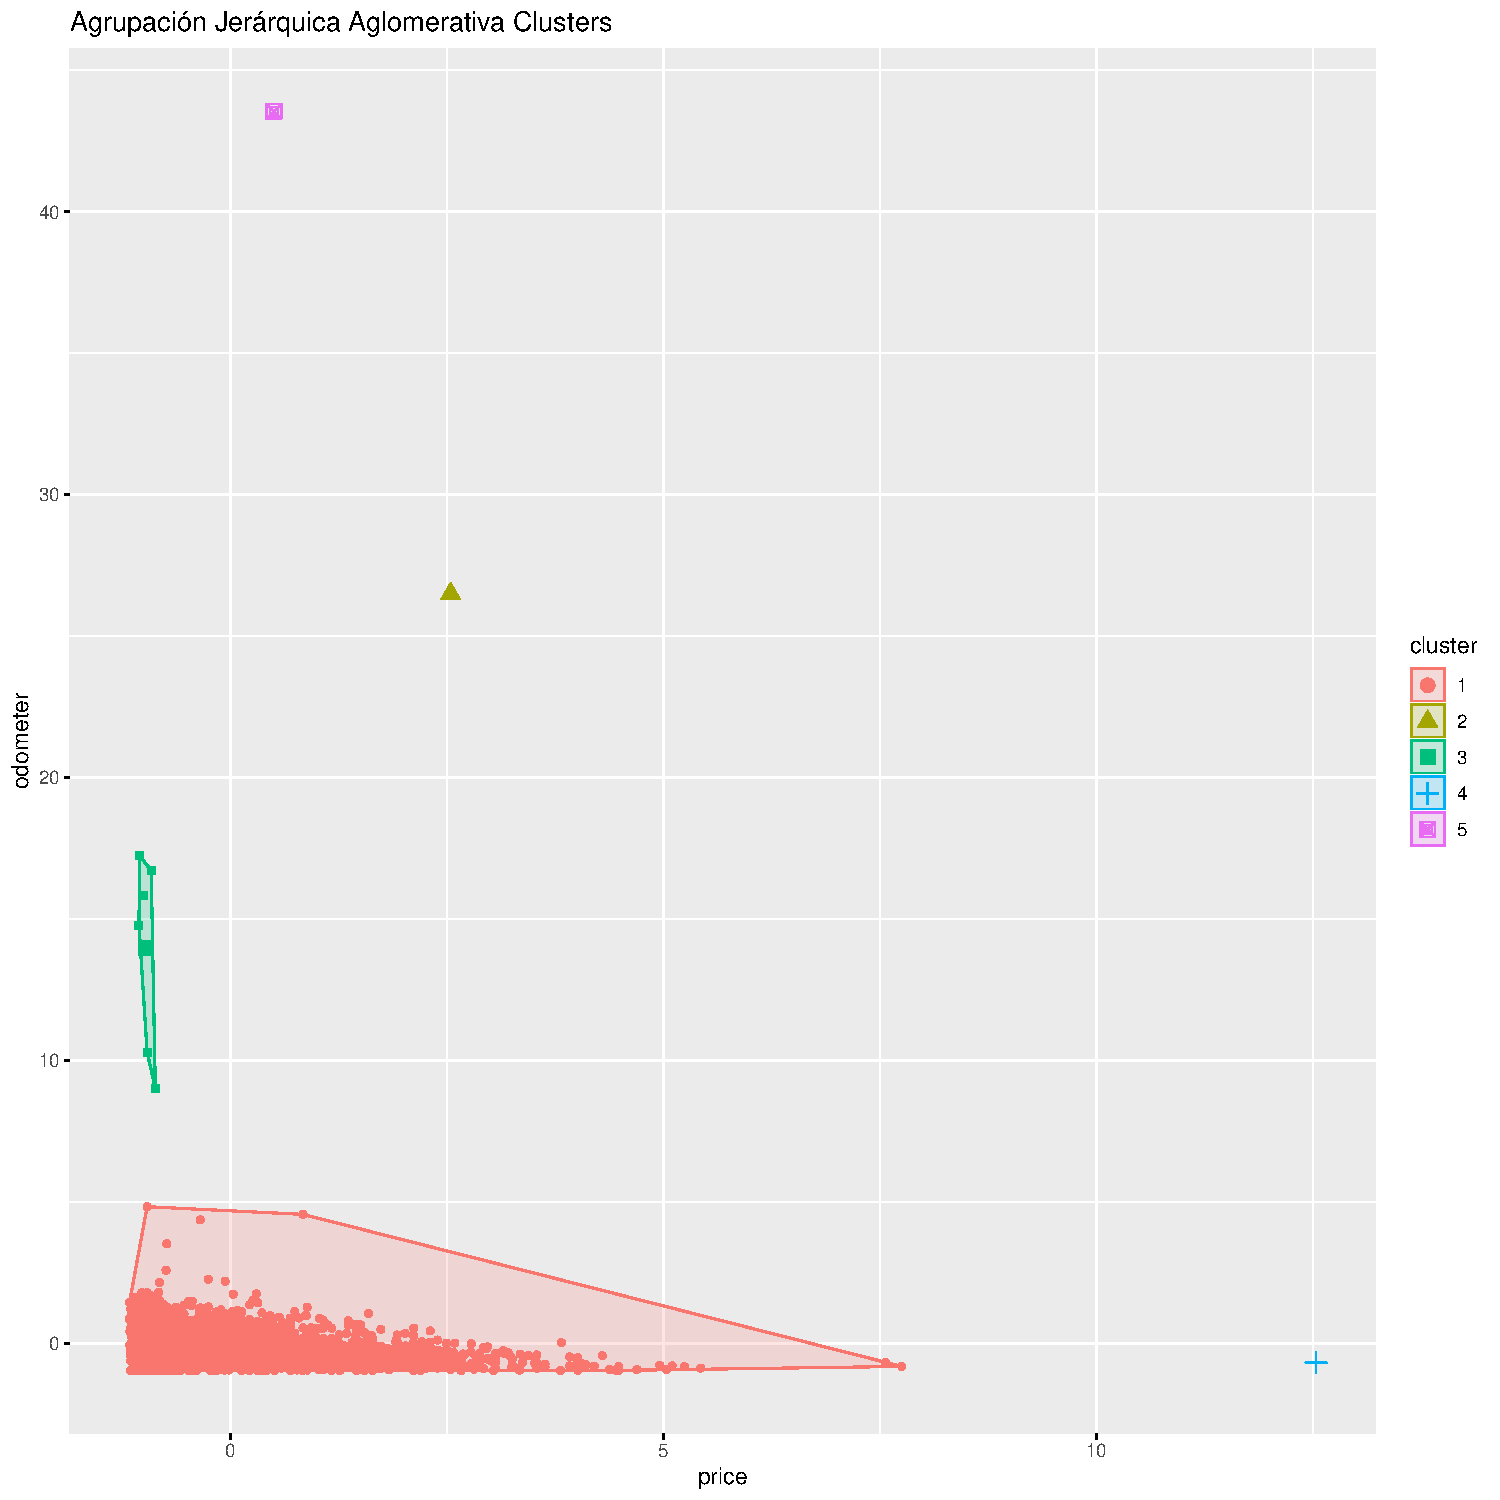
\includegraphics{Practica4-hc}

\subsection{K-Means jerárquico}
K-means es uno de los métodos de clustering que más se utilizan pero sufre las limitaciones de necesitar que se especifique el numero de clusters de antemano y que sus resultados puedan variar en funcion de la iniciación aleatoria. Una forma de hacer frente a estos problemas es combinando el K-means con la agrupación jerárquica, el procedimiento consiste en aplicar la agrupación jerárquica a los datos y cortar el arbol en k clusters en nuestro caso 4 ya que con más la gráfica no tiene los suficientes datos como para calcular una elipse, posteriormente se calcula el centro de cada cluster y finalmente se aplica el agrupamiento de k-means empleando como centroides iniciales los centros calculados anteriormente. Haremos uso de la función \textbf{hkmeans} para el cálculo. Imprimiremos los resultados en una gráfica con 4 clusters como ya se determinó previamente:

\begin{Schunk}
\begin{Sinput}
> set.seed(101)
> res.hk <-hkmeans(coches.normalizados, k=4)
\end{Sinput}
\end{Schunk}
\begin{Schunk}
\begin{Sinput}
> fviz_cluster(res.hk, geom = "point", main="K-means jerárquico")
\end{Sinput}
\end{Schunk}
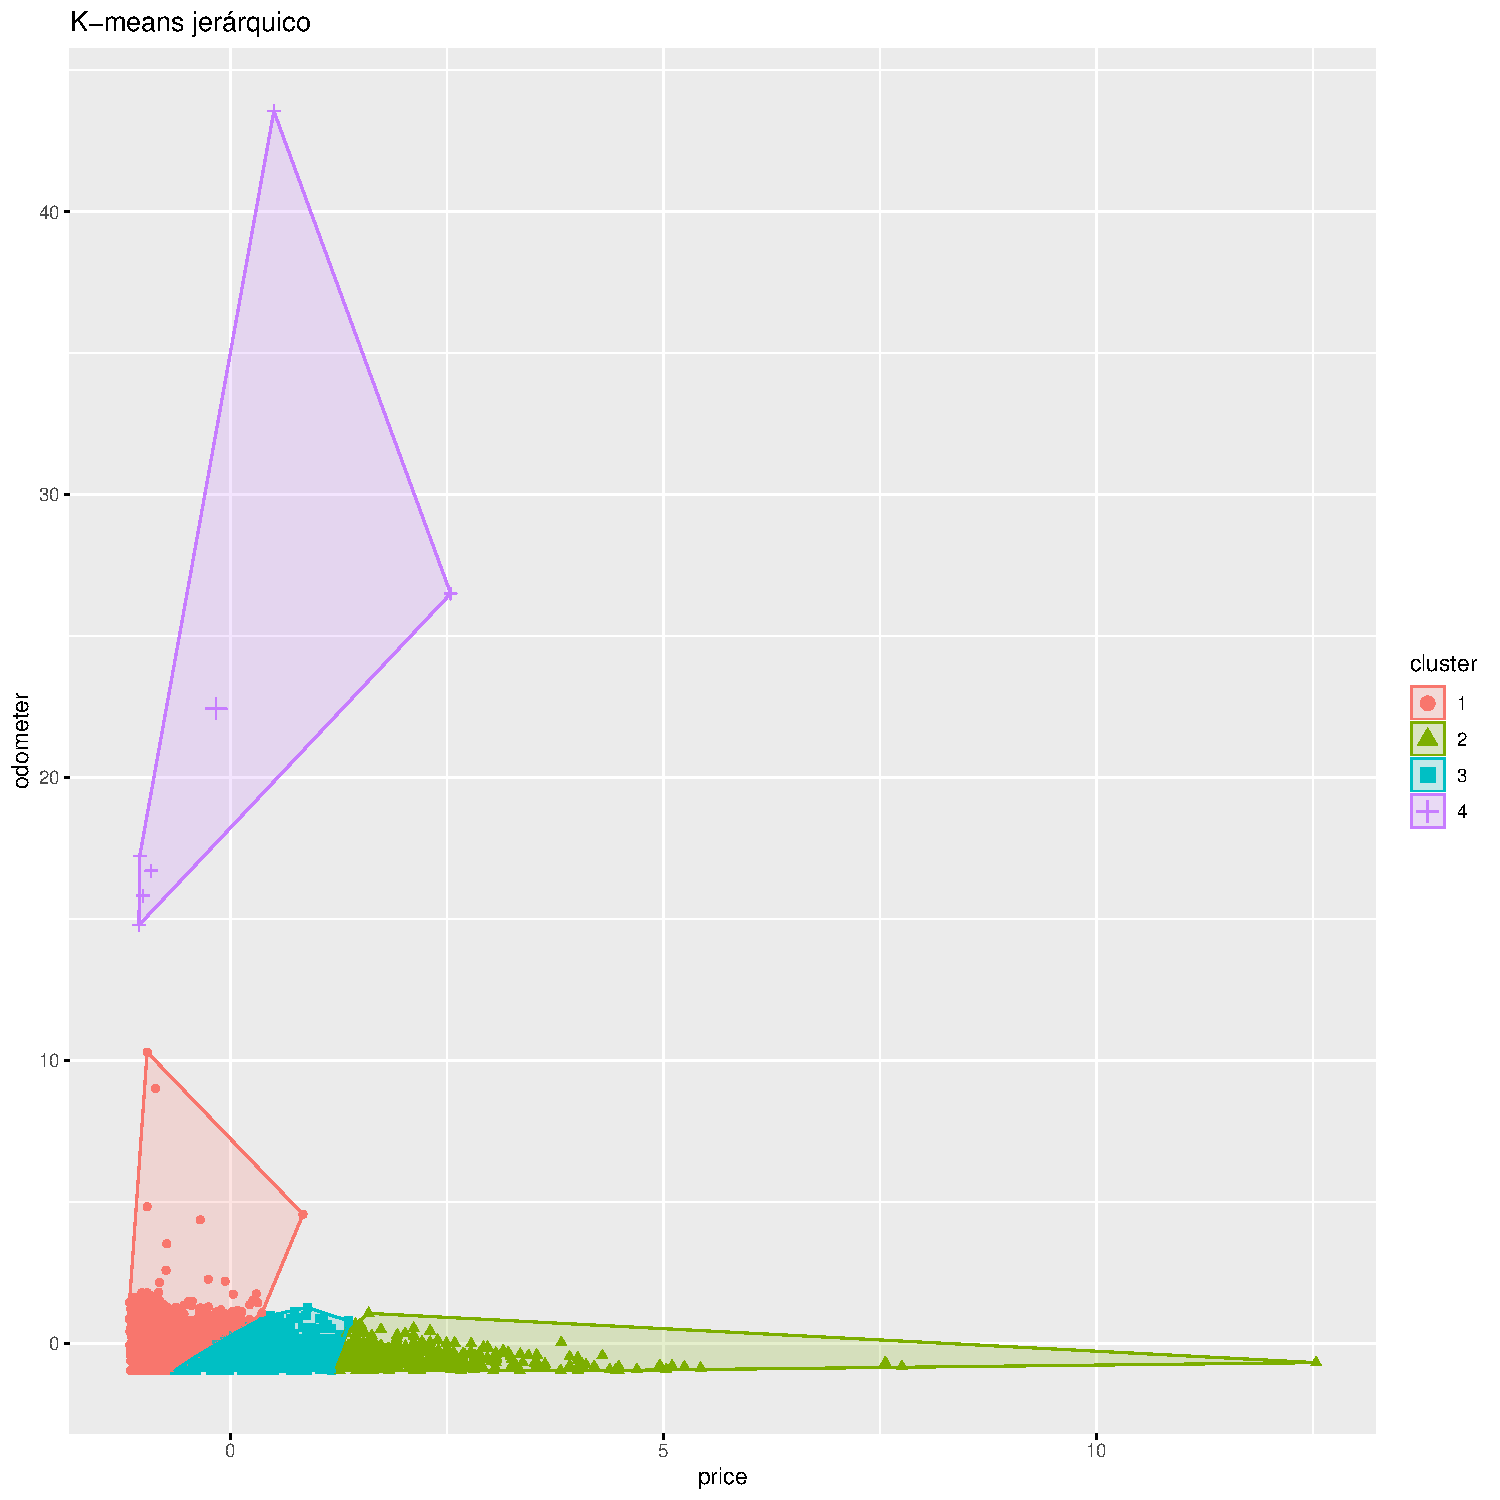
\includegraphics{Practica4-hk}

No empleamos dendogramas ya que la cantidad y el tipo de datos que estamos analizando nos genera muchos valores y las gráficas que se generan no aportan ninguna información clara.

\end{document}
